\documentclass[14pt]{mmcs-article}
\usepackage[russian]{babel}
\usepackage{amsmath, amsthm, amsfonts, amssymb}
\usepackage{listings, listings-rust}

% После кванторов ставить отступ
% Починить \mod (\mathsc) -- сейчас там большой пробел в начале

% Надо бы настроить правильную сквозную нумерацию замечаний, теорем e.t.c

\graphicspath{{paper_images/}}

\begin{document}

%см. РЕКОМЕНДАЦИИ ПО ОФОРМЛЕНИЮ
%И ПРЕДСТАВЛЕНИЮ КУРСОВЫХ И ВЫПУСКНЫХ %КВАЛИФИКАЦИОННЫХ РАБОТ СТУДЕНТОВ ИНСТИТУТА %МАТЕМАТИКИ, МЕХАНИКИ И КОМПЬЮТЕРНЫХ НАУК


% ----------------------------------
% Внимание!
% Изменяйте только строки, перед которыми стоят знаки комментариев
% ----------------------------------

\thispagestyle{empty}
\begin{singlespacing} 
\begin{center}

МИНОБРНАУКИ РОССИИ\\ [12pt]
Федеральное государственное автономное образовательное\\
учреждение высшего образования\\
<<Южный федеральный университет>>

\vspace{\baselineskip}
Институт математики, механики\\
и компьютерных наук им.~И.\,И.~Воровича


\vfill
% Фамилия Имя Отчество студента
\textbf{Арутюнов Олег Валентинович}

\vspace{15mm}
%НАЗВАНИЕ РАБОТЫ должно полностью соответствовать 
% приказу по ЮФУ (для выпускных квалификационных работ)
{\bf МЕТОДЫ ПОСТРОЕНИЯ (m,n)-РЕГУЛЯРНЫХ ДВУДОЛЬНЫХ ГРАФОВ С НАИБОЛЬШИМ ОБХВАТОМ }

\vspace{15mm}
ВЫПУСКНАЯ КВАЛИФИКАЦИОННАЯ РАБОТА\\
по направлению подготовки\\
% Направление обучения 
02.04.02 Фундаментальная информатика и информационные технологии,\\
направленность программы\\
<<Разработка мобильных приложений и компьютерных игр>>

\vspace{10mm}
\textbf{Научный руководитель~--}\\
% указать данные о руководителе
% должность, степень, звание Фамилия Имя Отчество
проф., д.\,ф.-м.\,н. Скороходов В. А.

% \vspace{7mm}
% \textbf{Рецензент~--}\\
% указать данные о рецензенте
% должность, степень, звание Фамилия Имя Отчество
% доц., к.\,т.\,н. Петров Иван Петрович


\vspace{15mm}

\noindent
% указать Фамилию и инициалы руководителя
% образовательной программы
\begin{flushleft}
Допущено к защите:\\
руководитель \\
образовательной программы \underline{\hspace*{60mm}} Демяненко Я.\,М.
\end{flushleft}




\vfill
% год!
Ростов-на-Дону -- 2024

\end{center} 

\singlespacing
\end{singlespacing}

\renewcommand{\contentsname}{Оглавление}

\tableofcontents

\newpage

\addcontentsline{toc}{section}{Введение}
\section*{Введение}

В описании современных стандартов передачи данных много внимания уделено контролю ошибок, неизбежно возникающими в любом канале связи. В теории кодирования применяют много различных подходов к проблеме коррекции подобных ошибок. Обычно для этого вместе с последовательностью данных передают последовательность проверочных битов, которые позволяют обнаружить и исправить ошибочно переданные сигналы. Примером таких алгоритмов могут служить алгоритм декодирования Земора \cite{zemor} и коды с малой плотностью проверок на чётность, так же известные как LDPC-коды \cite{johnson}.

Впервые LDPC-коды были описаны в работе Роберта Галагера \cite{gallager} в 1963 году, однако не применялись до 1996 года, из-за сложностей в реализации кодеров и декодеров.

LDPC-коды вошли в стандарт цифорвого спутникового вещания\\ DVB-S2, разработанный в 2003 году международным консорциумом DVB Project. Также LDPC коды включены в стандарты Ethernet 10GBASE-T и Wi-Fi 802.11.

Передача данных через канал с шумами осуществляется следующим образом: поток данных разбивают на блоки определённой длины, вместе с данными передаётся набор проверочных блоков, построенных на основе информационных блоков. Принимающая стороная использует проверочные блоки, чтобы убедиться в целостности данных в информационных блоках или восстановить допущенные ошибки, насколько это возможно.

Значение проверочных блоков в алгоритме LDPC вычисляется с помощью графа Таннера: вершины из одной доли соответствуют всем битам передаваемых данных, как непосредственно информации, так и данных, необходимых для проверки, вершины из второй доли соответствуют проверкам на чётность. Значение проверочных блоков выбирается таким образом, чтобы сумма всех вершин связанных с каждым узлом проверки на чётность равнялась нулю по модулю 2.
\\

\textbf{Пример.}

На рисунке \ref{tanner_example} изображён пример графа Таннера. Вершины, обозначающие проверки на чётность отмечен символом $+$, а информационные вершины ~-- значениями битов передаваемой информации. Значения проверочных вершин подобраны так, чтобы проверки на чётность не нарушались. 

\begin{figure}[H]
    \centering
    \begin{picture}(210,200)
        \put(50,165){\thicklines{\circle{20}}}
        \put(45,162){$+$}
        \put(110,165){\thicklines{\circle{20}}}
        \put(105,162){$+$}
        \put(170,165){\thicklines{\circle{20}}}
        \put(165,162){$+$}

        \put(35,35){\thicklines{\circle{20}}}
        \put(31,31){$1$}
        \put(65,35){\thicklines{\circle{20}}}
        \put(61,31){$0$}
        \put(95,35){\thicklines{\circle{20}}}
        \put(91,31){$1$}
        \put(125,35){\thicklines{\circle{20}}}
        \put(121,31){$0$}
        \put(155,35){\thicklines{\circle{20}}}
        \put(151,31){$1$}
        \put(185,35){\thicklines{\circle{20}}}
        \put(181,31){$1$}

        \bezier{300}(50,155)(42,100)(35,45)
        \bezier{300}(50,155)(57,100)(65,45)
        \bezier{300}(50,155)(72,100)(95,45)
        \bezier{300}(50,155)(87,100)(125,45)

        \bezier{300}(110,155)(102,100)(95,45)
        \bezier{300}(110,155)(117,100)(125,45)
        \bezier{300}(110,155)(147,100)(185,45)

        \bezier{300}(170,155)(102,100)(35,45)
        \bezier{300}(170,155)(147,100)(125,45)
        \bezier{300}(170,155)(162,100)(155,45)
    \end{picture}
    \caption{ Граф Таннера. }\label{tanner_example}
\end{figure}

От того, какими свойствами обладает используемый граф Таннера сильно зависит эффективность работы алгоритма LDPC. Поэтому активно ведутся исследования в области поиска методов построения графов Таннера с требуемыми параметрами.

Из эмпирических данных следует, что для наиболее успешного кодирования следует использовать графы с максимальным обхватом. На практике активно применяются графы с обхватом 12.

Методы построения таких графов, используемые в крупных компаниях, попадают под соглашения о неразглашении. Однако известны две основные группы методов: случайные, основанные на генерации начального графа случайным способом, например перебор возможных матриц \cite{bruteforce} и псевдослучайные пермутации матриц \cite{gallager}; и структурированные, основанные на построении графа с определённой, заранее известной структурой, например методы, использующие протографы \cite{protographs}.

Эмпирически показано, что лучшие результаты показывают графы, построенные случайными методами, однако структурированные методы позволяют получать коды с более предсказуемыми характеристиками, а так же оптимизировать хранение графов. 

В данной работе рассматриваются некоторые структурированные методы построения графов Таннера с заданными свойствами.

%=======================
\newpage
\addcontentsline{toc}{section}{Постановка задачи}

\section*{Постановка задачи}

% Прислать Владимиру Александроичу

Целью данной работы является разработка метода построения двудольных графов с заданным обхватом с помощью метаграфов. Для достижения цели выделяются несколько задач:

\begin{itemize}
  \item Произвести исследование структуры циклов в метаграфах. Разработать алгоритм поиска циклов наименьшей длины в метаграфах.
  \item Разработать метод нахождения весов дуг метаграфа для получения расширения с заданным обхватом.
  \item Разработать метод построения оптимальной структуры метаграфа.
  \item Провести вычислительный эксперимент для оценки характеристик полученных графов.
\end{itemize}

%=======================
\newpage
\section{Основные понятия и утверждения}

% Несколько общих слов о
Приведём определения основных понятий используемых далее [цитата].

\textbf{Определение 1.}

% Надо потом аккуратно в замечении это всё дело переопределить так, чтобы запись была более компактная (отказаться от отображения, использовать пары)

\textsl{Двудольным графом} будем называть тройку $ G(V, E, f)$, такую, что:

\begin{itemize}
    \item $V = A \cup B$ и $A \cap B = \emptyset$ ;
    % Возможно надо использовать неупорядоченное декартово произведение, о том как это лучше сделать, надо смотреть в книжке Зыкова
    \item $f: E \rightarrow A \times B$ ;
\end{itemize}

Где $V$ ~-- множество вершин, разбитое на два непересекающихся подмножества $A$ и $B$.
$E$ ~-- множество дуг.
$f$ ~-- это отображение, определяющее то, с какими вершинами инцидентна дуга.

\textbf{Определение 2.}

Последовательность дуг $\mu = (e_1, ..., e_d)$ будем называть путём с начальной вершиной $v_0$ и конечной вершиной $v_d$  на графе $G(V,E,f)$, если существует последовательность вершин $(v_0, ..., v_d)$ такая, что $\forall i = 1,...,d:$ $(v_i, v_{i+1}) = f(e_i)$ или $(v_{i+1}, v_i) = f(e_i)$. 

% Пронумеровать вершины

Рассмотрим граф на рис \ref{image:1}. Последовательность дуг $(e_1, e_2, e_4, e_6)$ составляет путь с начальной вершиной C и конечной вершиной E.

\begin{figure}[H]
    \centering
    \begin{picture}(220,200)
        \put(75,165){\thicklines{\circle*{5}}}
        \put(70,170){$c_1$}
        \put(35,35){\thicklines{\circle*{5}}}
        \put(30,20){$i_1$}
        \put(115,35){\thicklines{\circle*{5}}}
        \put(110,20){$i_2$}

        \thicklines
        \bezier{300}(75,165)(56,100)(35,35)
        \put(40,100){$e_1$}
        \bezier{300}(75,165)(94,100)(115,35)
        \put(80,100){$e_2$}
        \bezier{300}(175,165)(120,100)(115,35)
        \put(135,130){$e_4$}
        \bezier{300}(175,165)(194,100)(135,35)
        \put(165,60){$e_6$}

        \thinlines
        \bezier{300}(75,165)(130,100)(135,35)
        \put(105,130){$e_3$}

        \put(175,165){\thicklines{\circle*{5}}}
        \put(170,170){$c_1$}
        \put(135,35){\thicklines{\circle*{5}}}
        \put(130,20){$i_1$}
        \put(215,35){\thicklines{\circle*{5}}}
        \put(210,20){$i_2$}

        \bezier{300}(175,165)(156,100)(135,35)
        \put(140,100){$e_5$}
        \bezier{300}(175,165)(195,100)(215,35)
        \put(200,100){$e_7$}
    \end{picture}
    \caption{ Двудольный граф. }\label{image:1}
\end{figure}

\textbf{Определение 4.}

\textsl{Циклом} будем называть путь, у которого совпадают первая и последняя вершины.

\textbf{Определение 6.}

\textsl{Обхватом графа} называют длину его минимального цикла.

\textbf{Замечание 1.}

Отметим, что обхват любого двудольного графа является чётным числом

% большим, чем два.

\textbf{Замечание 2.}

Известно, что на практике для кодирования эффективнее использовать графы с большим обхватом.

\textbf{Определение 5.}

% Характеристика дуги внутри пути (в какую сторону путь проходит дугу)

С каждым путём $\mu$ свяжем характеристическую функцию $\chi_\mu(e)$:
\[
    \begin{array}{ll}
        \chi_{\mu}(e_1) = \left\{
            \begin{array}{ll}
            1,  & v_0 \in A;\\
            -1, & v_0 \in B. \\
            \end{array}
        \right. \\
        \chi_\mu(e_i) = -\chi_\mu(e_{i-1}) \forall i \in 2, ..., d\\
    \end{array}
\]

\section{Метаграфы}

% Несколько общих слов о метаграфах и, возможно, сразу и о расширениях
Далее будем рассматривать взвешенные графы такие что ..., которые будем называть метаграфами.

Дадим им формальное определение.

\textbf{Определение 6.}

Если $G(V,E,f)$ ~-- двудольный граф, то \textsl{Метаграфом} будем называть четвёрку $G'(V,E,f,w)$, где $w: E \to \mathbb{Z}$ ~-- отображения, задающее веса дуг.

На рис. \ref{image:2} представлен метаграф  $G_1$ с тремя вершинами и четырьмя дугами.

\begin{figure}[H]
    \centering
    \begin{picture}(150,200)
        \put(75,165){\thicklines{\circle*{5}}}
        \put(70,170){$c_1$}
    
        \put(35,35){\thicklines{\circle*{5}}}
        \put(30,20){$i_1$}
    
        \put(115,35){\thicklines{\circle*{5}}}
        \put(110,20){$i_2$}
    
        \bezier{300}(75,165)(10,100)(35,35)
        \put(5,100){$+1$}

        \bezier{300}(75,165)(56,100)(35,35)
        \put(56,80){$0$}
    
        \bezier{300}(75,165)(140,100)(115,35)
        \put(125,100){$-1$}

        \bezier{300}(75,165)(94,100)(115,35)
        \put(87,80){$0$}
    \end{picture}
    \caption{ Метаграф с весами дуг +1, 0, 0, -1.. }
    \label{image:2}
\end{figure}

\textbf{Определение 7.}

Пусть $r \in \mathbb{N}$, тогда $r$-расширением метаграфа $G'(V,E,f,w)$ назовём граф $G^{(r)}(V^{(r)}, E^{(r)}, f^{(r)})$ построенный следующим образом:

\begin{itemize}
    \item Каждой вершине $v \in V$ соответствует множество вершин
    \[
        T^{(r)}(v) = \{ v^{(1)}, ..., v^{(r)} \}
    \]

    \item Тогда множество вершин метаграфа устроено следующим образом 
    \[
        V^{(r)} = \bigcup_{v \in V} T^{(r)}(v)
    \]

    \item Каждой дуге $e \in E$ соответствует множество дуг 
    \[
        T^{(r)}(e) = \{ e^{(1)}, ..., e^{(r)} \}
    \]

    \item Тогда множество дуг метаграфа устроено следующим образом
    \[
        E^{(r)} = \bigcup_{e \in E}T^{(r)}(e)
    \]

    \item Пусть $f(e) = (a, b)$, тогда $f^{(r)}(e^{(i)}) = (a^{(i)}, b^{(i + w(e) (\mod{r}))}) \forall i = 1,...,r$
\end{itemize}

На рис. \ref{image:3} изображён граф, полученный 4-расширением метаграфа $G_1$, изображённого на рис. \ref{image:2}.
% Пример нужен, чтобы показать, что на метаграфах с кратными дугами яразу появляются маленькие циклы

\begin{figure}[H]
    \centering
    \begin{picture}(450,200)
        \put(75,165){\thicklines{\circle*{5}}}
        \put(70,170){$c_1$}
        \put(35,35){\thicklines{\circle*{5}}}
        \put(30,20){$i_1$}
        \put(115,35){\thicklines{\circle*{5}}}
        \put(110,20){$i_2$}

        \bezier{300}(75,165)(56,100)(35,35)
        \bezier{300}(75,165)(94,100)(115,35)
        \bezier{300}(75,165)(130,100)(135,35)
        \bezier{300}(175,165)(120,100)(115,35)

        \put(175,165){\thicklines{\circle*{5}}}
        \put(170,170){$c_1$}
        \put(135,35){\thicklines{\circle*{5}}}
        \put(130,20){$i_1$}
        \put(215,35){\thicklines{\circle*{5}}}
        \put(210,20){$i_2$}

        \bezier{300}(175,165)(156,100)(135,35)
        \bezier{300}(175,165)(194,100)(215,35)
        \bezier{300}(175,165)(230,100)(235,35)
        \bezier{300}(275,165)(220,100)(215,35)


        \put(275,165){\thicklines{\circle*{5}}}
        \put(270,170){$c_1$}
        \put(235,35){\thicklines{\circle*{5}}}
        \put(230,20){$i_1$}
        \put(315,35){\thicklines{\circle*{5}}}
        \put(310,20){$i_2$}

        \bezier{300}(275,165)(256,100)(235,35)
        \bezier{300}(275,165)(294,100)(315,35)
        \bezier{300}(275,165)(330,100)(335,35)
        \bezier{300}(375,165)(320,100)(315,35)


        \put(375,165){\thicklines{\circle*{5}}}
        \put(370,170){$c_1$}
        \put(335,35){\thicklines{\circle*{5}}}
        \put(330,20){$i_1$}
        \put(415,35){\thicklines{\circle*{5}}}
        \put(410,20){$i_2$}

        \bezier{300}(375,165)(356,100)(335,35)
        \bezier{300}(375,165)(394,100)(415,35)

        \bezier{700}(75,165)(245,100)(415,35)
        \bezier{700}(375,165)(205,100)(35,35)
    \end{picture}
    \caption{ Метаграф с весами дуг +1, 0, 0, -1.. }
    \label{image:3}
\end{figure}

\textbf{Теорема 1.} \textsl{(О начальных вершинах путей)}

Пусть $\eta = (e_1, \dots, e_d)$ ~-- путь с начальной вершиной $v$ на метаграфе $G$, тогда на графе $G^{(r)}$ существуют $r$ попарно не пересекающихся путей $\mu_1 \dots \mu_r$ с начальными вершинами $v^{(1)}, ..., v^{(r)}$, таких что для каждого пути $\mu'=(e_1',\dots,e_d') \in\{\mu_1,\dots,\mu_r\}$ справедливо, что для всех $j\in[1;d]_N$ $e_{j}' \in T^{(r)}(e_j)$.

\textbf{Доказательство.}

% Skorokhodov V.A. Generalization of the Reachability Problem on Directed Graphs/ Mathematics and Statistics, Vol. 8, No. 6, pp. 699 - 704, 2020. DOI: 10.13189/ms.2020.080610

Следует из определения расширения метаграфа.

\qed

\textbf{Определение 8.}

Будем говорить, что пути $\eta$ на метаграфе $G$ соответствуют пути $\mu_i$ на графе $G^{(r)}$ и наоборот.

\textbf{Замечание 2.}

Из того, что некоторый путь на метаграфе $G$ является циклом не следует, что соответствующие ему пути на $G^{(r)}$ являются циклами. Рассмотрим эту ситуацию на следующем примере.

\textbf{Пример 1.}

Рассмотрим граф на рис. \ref{image:4}. Путь $(e_1, e_2)$ является циклом на метаграфе, однако ни один из соответствующих ему путей $\mu_1 = (e^{(1)}_1, e^{(1)}_2)$, $\mu_2 = (e^{(2)}_1, e^{(2)}_2)$, $\mu_3 = (e^{(3)}_1, e^{(3)}_2)$  на 3-расширении не является циклом. При этом следует отметить, что склейка этих трёх путей порождает цикл $\mu = (e^{(1)}_1, e^{(1)}_2, e^{(2)}_1, e^{(2)}_2, e^{(3)}_1, e^{(3)}_2)$ длины 6. Заметим, что циклу $\mu$ соответствует цикл $(e_1, e_2, e_1, e_2, e_1, e_2)$ на метаграфе.

\begin{figure}[H]
    \centering
    \begin{picture}(255,200)
        \put(0,165){$a.$}

        \put(35,165){\thicklines{\circle*{5}}}
        \put(30,170){$A$}
        \put(35,35){\thicklines{\circle*{5}}}
        \put(30,20){$B$}
    
        \bezier{300}(35,165)(10,100)(35,35)
        \put(0,100){$e_1$}
        \bezier{300}(35,165)(60,100)(35,35)
        \put(56,100){$e_ 2$}



        \put(110,165){$b.$}

        \put(145,165){\thicklines{\circle*{5}}}
        \put(140,170){$A^{(1)}$}
        \put(145,35){\thicklines{\circle*{5}}}
        \put(140,20){$B^{(1)}$}

        \thicklines
        \bezier{300}(145,165)(145,100)(145,35)
        \put(125,130){$e_0^{(1)}$}

        \bezier{300}(145,165)(165,100)(185,35)
        \put(147,85){$e_1^{(1)}$}
        \thinlines

        \put(185,165){\thicklines{\circle*{5}}}
        \put(180,170){$A^{(2)}$}
        \put(185,35){\thicklines{\circle*{5}}}
        \put(180,20){$B^{(2)}$}

        \bezier{300}(185,165)(185,100)(185,35)
        \put(165,130){$e_0^{(2)}$}
        
        \bezier{300}(185,165)(205,100)(225,35)
        \put(187,85){$e_1^{(2)}$}

        \put(225,165){\thicklines{\circle*{5}}}
        \put(220,170){$A^{(3)}$}
        \put(225,35){\thicklines{\circle*{5}}}
        \put(220,20){$B^{(3)}$}

        \bezier{300}(225,165)(225,100)(225,35)
        \put(205,130){$e_0^{(3)}$}

        \bezier{300}(225,165)(232,50)(145,35)
        \put(190,45){$e_1^{(3)}$}
    \end{picture}
    \caption{ a. Метаграф. b. 3-расширение метаграфа. }
    \label{image:2}
\end{figure}

\textbf{Определение 7.}

Пусть $G(V, E, f, w)$ ~-- метаграф.

Характеристикой пути $\eta = (e_1, ..., e_d)$ будем называть

\[
    \chi(\eta) = \sum_{i = 1}^d \chi_{\eta}(e_i) w(e_i).
\]

\textbf{Теорема 2.}\textsl{(О конечных вершинах путей)}

Пусть  $\eta = (e_1, ..., e_d)$ ~-- путь на метаграфе $G$, его первая вершина ~-- $x$, а последняя вершина ~-- $y$. И пусть $\mu' = (e'_1, ..., e'_d)$ один из соответствующих ему путей на расширенном графе.

Тогда если у $\mu'$ начальная вершина $x^{(i)}$, то его последняя вершина ~-- $y^{(i + \chi(\eta)\mod{r})}$.

\textbf{Доказательство.}

% Как-то лучше мы это переписывали, а то просто месиво символов получается. Может там чуть ли не на "очевидно" можно было заменить

Доказательство проведём по индукции по длине пути $|\eta| = d$.

Пусть $d = 1$, тогда путь состоит их одной дуги $e_1$.

Если $x \in A$, тогда вершина $x^{(i)}$ инцидентна дуге $e_1'$, для которой $f^{(r)}(e_1') = (x^{(i)}, y^{(i + w(e_1) (\mod{r}))})$ то есть, конечной вершиной пути $\mu_i$ является $y^{(i + w(e_1) (\mod{r}))} = y^{(i + \chi(\eta) (\mod{r}))}$.

Если $x \in B$, тогда вершина $x^{(i)}$ инцидентна дуге $e_1'$, для которой $f^{(r)}(e_1') = (y^{(i - w(e_1) (\mod{r}))}, x^{(i)})$ то есть, конечной вершиной пути $\mu_i$ является $y^{(i - w(e_1) (\mod{r}))} = y^{(i + \chi(\eta) (\mod{r}))}$.

Пусть условия теоремы выполняются для всякого $d < n$, тогда рассмотрим случай $d = n$.

Рассмотрим путь $\eta' = (e_1, ..., e_{d - 1})$. Обозначим его последнюю вершину $x$. Тогда по предположению индукции последние вершины соответствующих ему путей на метаграфе ~-- это $x^{(i + \chi(\eta')(\mod{r}))}$.

Если $x \in A$, тогда вершина $x^{(i + \chi(\eta')(\mod{r}))}$ инцидентна дуге \\ $f^{(r)}(e_d^{(i + \chi(\eta')(\mod{r}))}) = (x^{(i + \chi(\eta')(\mod{r}))}, y^{(i + \chi(\eta') + w(e_d) (\mod{r}))})$ и конечная \\ вершина пути $\mu_i$ ~-- $y^{(i + \chi(\eta') + w(e_d) (\mod{r}))} = y^{(i + \chi(\mu) (\mod{r}))}$.

Если $x \in B$, тогда вершина $x^{(i + \chi(\eta')(\mod{r}))}$ инцидентна дуге \\ $f^{(r)}(e_d^{(i + \chi(\eta') - w(e_d) (\mod{r}))}) = (y^{(i + \chi(\eta') - w(e_d) (\mod{r}))}, x^{(i)})$ и конечная вершина пути $\mu_i$ ~-- $y^{(i + \chi(\eta') - w(e_d) (\mod{r}))} = y^{(i + \chi(\mu) (\mod{r}))}$.

\qed

Важными следствиями из Теоремы 2 являются две следующих теоремы.

\textbf{Теорема 3.} \textsl{(О циклах)}

Пусть $\eta$ ~-- цикл на метаграфе. Тогда соответствующие ему пути на расширенном графе являются циклами тогда и только тогда, когда $\chi(\eta) = 0 (\mod{r})$.

\textbf{Теорема 4.} \textsl{(О <<крыльях>> цикла)}

Пусть $\eta = (e_1, ..., e_d)$ и $\mu = (\epsilon_1, ..., \epsilon_{\delta})$ ~-- различные пути на метаграфе с начальной вершиной $a$, конечной вершиной $b$ и $\chi(\eta) = \chi(\mu) (\mod{r})$. Тогда путь на расширении, соответствующий склейке этих путей \\ $\gamma = (e_1, \dots, e_d, \epsilon_{\delta}, \dots, \epsilon_1)$, является циклом.

Эти теоремы дают метод нахождения циклов на расширенном графе, описываемый следующим алгоритмом:

%%%%%%%%% Всё что выше не переписываем (пока что)

\textbf{Алгоритм 1.}

Поиска цикла с длинной меньше или равной заданному чётному числу $l \in \mathbb{N}$.

Пусть $G(A \cup B, E, f, w)$ ~-- метаграф и задано $r \in \mathbb{N}$.

Алгоритм основан на заполнении множества меток для вершин метаграфа. Каждая метка представляет собой четвёрку $(g, v, ch, p)$, где $g$ ~-- длина пути $\mu$ пройденного от начальной до помечаемой вершины, далее $g$ будем называть поколением метки; $v$ ~-- вершина, которая помечена этой меткой; $ch \in \mathbb{Z}$ ~-- характеристика метки, обозначает характеристику пути $\mu$; $p \in V \cup \{ nil \}$ ~-- дуга, на основе которой была сгенерирована метка, при обработке предыдущего поколения меток, где $nil \not\in V $ ~-- специальное значение, зарезервированное для исходной метки.

\begin{itemize}

\item Для каждой вершины $a \in A:$

\begin{itemize}
    \item Добавим метку $(0, a, 0, nil)$ в пустое множество всех меток
    \item В цикле по поколениям $g$ от $1$ до $l / 2$:
    \begin{itemize}
        \item Для всех меток вида $(g - 1, v, ch, p)$:
        \item
            Для каждой дуги $e \not= p$ инцидентной вершине $v$,
            формируем метку $(g, v', ch', e)$, где $ch' = ch + (-1)^{g} w(e) (\mod{r})$, $v'$ ~-- вершина отличная от $v$, инцидентная $e$.
            Добавляем эту метку ко множеству всех меток.
    \end{itemize}
    \item Если существуют хотя бы две метки с совпадающими вторым и третьим элементами, сообщаем о том, что обнаружен цикл и завершаем работу алгоритма.
\end{itemize}

\item Сообщаем о том, что цикл не найден.
\end{itemize}

\textbf{Пример 2.}

% Возможно лучше разделить на два отедельынх рисунка и ссылаться по отдельности

Рассмотрим этапы поиска цикла на метаграфе, изображённом на рис. \ref{cycle_search}, с помощью алгоритма 1. В таблице \ref{cycle_search_table} приведено множество меток, сгенерированных алгоритмом для начальной вершины $v_1$, сгруппированное в столбцы по поколению.

\begin{figure}[H]
    \centering
    \begin{picture}(170,200)
        \put(35,165){\thicklines{\circle*{5}}}
        \put(30,170){$v_1$}
        \put(115,165){\thicklines{\circle*{5}}}
        \put(110,170){$v_2$}

        \put(35,35){\thicklines{\circle*{5}}}
        \put(30,20){$v_3$}
        \put(115,35){\thicklines{\circle*{5}}}
        \put(110,20){$v_4$}

        \bezier{300}(35,165)(-10,100)(35,35)
        \put(0,100){$a$}
        \bezier{300}(35,165)(35,100)(35,35)
        \put(40,100){$b$}
        \bezier{300}(35,165)(70,100)(115,35)
        \put(60,130){$c$}

        \bezier{300}(115,165)(115,100)(115,35)
        \put(120,100){$e$}
        
        \bezier{300}(115,165)(70,100)(35,35)
        \put(80,130){$d$}
    \end{picture} \\
    \begin{tabular}{ | c | c | }
        \hline
        $e$ & $w(e)$ \\ \hline
        $a$ & $-1$   \\
        $b$ & $0$    \\
        $c$ & $+1$   \\
        $d$ & $0$    \\
        $e$ & $0$    \\ \hline
    \end{tabular}
    \caption{ Пример метаграфа. }\label{cycle_search}
\end{figure}

В поколении 3 есть метки $(3, v_4,  0, c)$ и $(3, v_4,  0, e)$, у которых совпадают второй и третий элементы. Следовательно, цикл найден. Отметим, что длина этого цикла на расширении метаграфа равна $6$ ~-- сумме поколений этих двух меток. 

\begin{table}[H]
    \centering
    \begin{tabular}{ | c | c | c | c | }
        \hline
        $g = 0$            & $g = 1$           & $g = 2$           & $g = 3$ \\ \hline
        $(0, v_1, 0, nil)$ & $(1, v_3,  0, b)$ & $(2, v_1,  4, b)$ & $(3, v_3,  3, a)$ \\ \hline
                           & $(1, v_3,  4, a)$ & $(2, v_1,  1, a)$ & $(3, v_4,  0, c)$ \\ \hline
                           & $(1, v_4,  1, c)$ & $(2, v_2,  1, e)$ & $(3, v_3,  0, a)$ \\ \hline
                           &                   & $(2, v_2,  0, d)$ & $(3, v_4,  2, c)$ \\ \hline
                           &                   & $(2, v_2,  4, d)$ & $(3, v_3,  1, d)$ \\ \hline
                           &                   &                   & $(3, v_4,  0, e)$ \\ \hline
                           &                   &                   & $(3, v_4,  4, e)$ \\ \hline
    \end{tabular}
    \caption{ Множество меток, сгенерированное в процессе работы алгоритма поиска цикла на метаграфе. }
    \label{cycle_search_table}
\end{table}

На рис. \ref{cycle_search_expanded} изображено 5-расширение метаграфа изображённого на рис. \ref{cycle_search}. Цикл, соответствующий найденному в ходе работы алгоритма выделен жирным. % (Когда будет конечная версия рисунка -- заменить)

\begin{figure}[H]
    \centering
    \begin{picture}(360,250)
        \put(35,165){\thicklines{\circle*{5}}}
        \put(65,165){\thicklines{\circle*{5}}}
        \put(35,35){\thicklines{\circle*{5}}}
        \put(65,35){\thicklines{\circle*{5}}}

        \bezier{300}(65,165)(65,100)(65,35)
        \bezier{300}(65,165)(50,100)(35,35)


        \thicklines
        \bezier{300}(35,165)(85,100)(135,35)
        \bezier{300}(35,165)(35,100)(35,35)
        \bezier{300}(105,165)(70,100)(35,35)
        \thinlines

        \put(105,165){\thicklines{\circle*{5}}}
        \put(135,165){\thicklines{\circle*{5}}}
        \put(105,35){\thicklines{\circle*{5}}}
        \put(135,35){\thicklines{\circle*{5}}}

        \thicklines
        \bezier{300}(105,165)(105,100)(105,35)
        \bezier{300}(135,165)(135,100)(135,35)
        \bezier{300}(135,165)(120,100)(105,35)
        \thinlines

        \bezier{300}(105,165)(155,100)(205,35)
        \bezier{300}(175,165)(140,100)(105,35)

        \put(175,165){\thicklines{\circle*{5}}}
        \put(205,165){\thicklines{\circle*{5}}}
        \put(175,35){\thicklines{\circle*{5}}}
        \put(205,35){\thicklines{\circle*{5}}}

        \bezier{300}(175,165)(175,100)(175,35)
        \bezier{300}(205,165)(205,100)(205,35)
        \bezier{300}(205,165)(190,100)(175,35)

        \bezier{300}(175,165)(225,100)(275,35)
        \bezier{300}(245,165)(210,100)(175,35)

        \put(245,165){\thicklines{\circle*{5}}}
        \put(275,165){\thicklines{\circle*{5}}}
        \put(245,35){\thicklines{\circle*{5}}}
        \put(275,35){\thicklines{\circle*{5}}}

        \bezier{300}(245,165)(245,100)(245,35)
        \bezier{300}(275,165)(275,100)(275,35)
        \bezier{300}(275,165)(260,100)(245,35)

        \bezier{300}(245,165)(295,100)(345,35)
        \bezier{300}(315,165)(280,100)(245,35)

        \put(315,165){\thicklines{\circle*{5}}}
        \put(345,165){\thicklines{\circle*{5}}}
        \put(315,35){\thicklines{\circle*{5}}}
        \put(345,35){\thicklines{\circle*{5}}}

        \bezier{300}(315,165)(315,100)(315,35)
        \bezier{300}(345,165)(345,100)(345,35)
        \bezier{300}(345,165)(330,100)(315,35)

        \bezier{700}(315,165)(65,275)(65,35)
        \bezier{700}(315,165)(35,325)(35,35)
    \end{picture}
    \caption{ 5-расширение метаграфа. }\label{cycle_search_expanded}
\end{figure}


\textbf{Замечание.}

Если в алгоритме 1.  учитывать совпадающие характеристики только пометок в текущем поколении, ты будут найдены только циклы состоящие из двух <<крыльев>> одинаковой длины, однако любой цикл на метаграфе представим в таком виде, следовательно будут найдены все циклы.

\textbf{Пример 3.}

Рассмотрим ещё один пример работы алгоритма на рис. \ref{cycle_mod_search}. В верхней части изображён метаграф $G$, в нижней части ~-- отображение из дуг в веса. В таблице. \ref{cycle_search_mod_table} приведено множество меток, сгенерированных алгоритмом для начальной вершины $v_1$. На рисунке \ref{cycle_search_mod_expanded} изображено 6-расширение метаграфа $G$, на котором помечен найденный цикл, который проходит по кругу через весь граф.

\begin{figure}[H]
    \centering
    % \begin{hbox}
    \begin{picture}(170,200)
        \put(35,165){\thicklines{\circle*{5}}}
        \put(30,170){$v_1$}
        \put(115,165){\thicklines{\circle*{5}}}
        \put(110,170){$v_2$}

        \put(35,35){\thicklines{\circle*{5}}}
        \put(30,20){$v_3$}
        \put(115,35){\thicklines{\circle*{5}}}
        \put(110,20){$v_4$}

        \bezier{300}(35,165)(35,100)(35,35)
        \put(40,100){$a$}
        \bezier{300}(35,165)(75,100)(115,35)
        \put(60,130){$b$}

        \bezier{300}(115,165)(75,100)(35,35)
        \put(80,130){$c$}
        \bezier{300}(115,165)(115,100)(115,35)
        \put(120,100){$d$}
    \end{picture} \\
    \begin{tabular}{ | c | c | }
        \hline
        $e$ & $w(e)$ \\ \hline
        $a$ & $+1$   \\
        $b$ & $0$    \\
        $c$ & $-1$   \\
        $d$ & $+1$   \\ \hline
    \end{tabular}
    % \end{hbox}
    \caption{ Пример метаграфа. }\label{cycle_mod_search}
\end{figure}

\begin{table}[H]
    \centering
    \begin{tabular}{ | c | c | c | c | c | }
        \hline
        $g = 0$            & $g = 1$           & $g = 2$           & $g = 3$           & $g = 4$            \\ \hline
        $(0, v_1, 0, nil)$ & $(1, v_3,  1, a)$ & $(2, v_2,  2, c)$ & $(3, v_4,  3, a)$ & $(3, v_1,  3, b)$  \\ \hline
                           & $(1, v_4,  0, b)$ & $(2, v_2,  5, d)$ & $(3, v_3,  4, c)$ & $(3, v_1,  3, a)$  \\ \hline
    \end{tabular}
    \caption{ Множество меток, сгенерированное в процессе работы алгоритма поиска цикла на метаграфе. }
    \label{cycle_search_mod_table}
\end{table}

\begin{figure}[H]
    \centering
    \begin{picture}(420,200)
        \put(35,165){\thicklines{\circle*{5}}}
        \put(65,165){\thicklines{\circle*{5}}}
        \put(35,35){\thicklines{\circle*{5}}}
        \put(65,35){\thicklines{\circle*{5}}}

        \bezier{300}(35,165)(70,100)(105,35)
        \bezier{300}(65,165)(100,100)(135,35)
        \bezier{300}(35,165)(50,100)(65,35)

        \put(105,165){\thicklines{\circle*{5}}}
        \put(135,165){\thicklines{\circle*{5}}}
        \put(105,35){\thicklines{\circle*{5}}}
        \put(135,35){\thicklines{\circle*{5}}}

        \bezier{300}(105,165)(140,100)(175,35)
        \bezier{300}(105,165)(120,100)(135,35)
        \bezier{300}(205,165)(155,100)(105,35)


        \put(175,165){\thicklines{\circle*{5}}}
        \put(205,165){\thicklines{\circle*{5}}}
        \put(175,35){\thicklines{\circle*{5}}}
        \put(205,35){\thicklines{\circle*{5}}}

        \bezier{300}(205,165)(240,100)(275,35)
        \bezier{300}(275,165)(225,100)(175,35)


        \put(245,165){\thicklines{\circle*{5}}}
        \put(275,165){\thicklines{\circle*{5}}}
        \put(245,35){\thicklines{\circle*{5}}}
        \put(275,35){\thicklines{\circle*{5}}}

        \bezier{300}(245,165)(280,100)(315,35)
        \bezier{300}(275,165)(310,100)(345,35)
        \bezier{300}(245,165)(260,100)(275,35)


        \put(315,165){\thicklines{\circle*{5}}}
        \put(345,165){\thicklines{\circle*{5}}}
        \put(315,35){\thicklines{\circle*{5}}}
        \put(345,35){\thicklines{\circle*{5}}}

        \bezier{300}(315,165)(350,100)(385,35)
        \bezier{300}(315,165)(330,100)(345,35)
        \bezier{300}(415,165)(365,100)(315,35)


        \put(385,165){\thicklines{\circle*{5}}}
        \put(415,165){\thicklines{\circle*{5}}}
        \put(385,35){\thicklines{\circle*{5}}}
        \put(415,35){\thicklines{\circle*{5}}}

        \thicklines
        \bezier{600}(385,165)(215,70)(35,35)
        \bezier{300}(135,165)(85,100)(35,35)
        \bezier{300}(135,165)(170,100)(205,35)
        \bezier{300}(175,165)(190,100)(205,35)
        \bezier{300}(175,165)(210,100)(245,35)
        \bezier{300}(345,165)(295,100)(245,35)
        \bezier{300}(345,165)(380,100)(415,35)
        \bezier{300}(385,165)(400,100)(415,35)
        \thinlines

        \bezier{600}(415,165)(245,70)(65,35)
        \bezier{600}(65,165)(225,130)(385,35)

    \end{picture}
    \caption{ 6-расширение метаграфа. }\label{cycle_search_mod_expanded}
\end{figure}

\textbf{Замечание.}

Сравним циклы, выделенные на рисунках \ref{cycle_search_expanded} и \ref{cycle_search_mod_expanded}. Цикл на первом рисунке будет иметь длину 6 вне зависимости от того, какое число $r$ мы выберем для r-расширения, в то время как цикл на втором рисунке пропадёт, если выбрать $r > 6$.

Цикл на метаграфе не зависит от выбранного $r$ в том случае, когда характеристики меток будут равны даже при сравнении без модуля.

На рисунке \ref{cycle_search_expanded_extra} изображено r-расширение метаграфа с рисунка \ref{cycle_search} с неким большим $r$. Часть компонент этого графа опущена, и обозначена многоточием. Заметим, что увеличение $r$ не привело к увеличению выделенного цикла.

\begin{figure}[H]
    \centering
    \begin{picture}(440,200)

        \put(35,100){\thinlines{\circle{3}}}
        \put(45,100){\thinlines{\circle{3}}}
        \put(55,100){\thinlines{\circle{3}}}

        \bezier{300}(135,35)(135,35)(65,120)
        \bezier{300}(105,165)(105,165)(65,100)

        \put(105,165){\thicklines{\circle*{5}}}
        \put(135,165){\thicklines{\circle*{5}}}
        \put(105,35){\thicklines{\circle*{5}}}
        \put(135,35){\thicklines{\circle*{5}}}

        \thicklines
        \bezier{300}(105,165)(105,100)(105,35)
        \thinlines
        \bezier{300}(135,165)(135,100)(135,35)
        \bezier{300}(135,165)(120,100)(105,35)

        \thicklines
        \bezier{300}(105,165)(155,100)(205,35)
        \bezier{300}(175,165)(140,100)(105,35)
        \thinlines

        \put(175,165){\thicklines{\circle*{5}}}
        \put(205,165){\thicklines{\circle*{5}}}
        \put(175,35){\thicklines{\circle*{5}}}
        \put(205,35){\thicklines{\circle*{5}}}

        \thicklines
        \bezier{300}(175,165)(175,100)(175,35)
        \bezier{300}(205,165)(205,100)(205,35)
        \bezier{300}(205,165)(190,100)(175,35)
        \thinlines

        \bezier{300}(175,165)(225,100)(275,35)
        \bezier{300}(245,165)(210,100)(175,35)

        \put(245,165){\thicklines{\circle*{5}}}
        \put(275,165){\thicklines{\circle*{5}}}
        \put(245,35){\thicklines{\circle*{5}}}
        \put(275,35){\thicklines{\circle*{5}}}

        \bezier{300}(245,165)(245,100)(245,35)
        \bezier{300}(275,165)(275,100)(275,35)
        \bezier{300}(275,165)(260,100)(245,35)

        \bezier{300}(245,165)(295,100)(345,35)
        \bezier{300}(315,165)(280,100)(245,35)

        \put(315,165){\thicklines{\circle*{5}}}
        \put(345,165){\thicklines{\circle*{5}}}
        \put(315,35){\thicklines{\circle*{5}}}
        \put(345,35){\thicklines{\circle*{5}}}

        \bezier{300}(315,165)(315,100)(315,35)
        \bezier{300}(345,165)(345,100)(345,35)
        \bezier{300}(345,165)(330,100)(315,35)

        \bezier{200}(345,165)(345,165)(385,115)
        \bezier{300}(385,165)(350,100)(315,35)

        \put(390,100){\thinlines{\circle{3}}}
        \put(400,100){\thinlines{\circle{3}}}
        \put(410,100){\thinlines{\circle{3}}}
    \end{picture}
    \caption{ Разомкнутое расширение метаграфа с независящим от r циклом. }\label{cycle_search_expanded_extra}
\end{figure}

Цикл, зависящий от $r$ пропадает, если выбрать больший $r$, однако в таком случае возникнет больший цикл так же проходящий по кругу через весь граф.

\begin{figure}[H]
    \centering
    \begin{picture}(420,200)
        \put(-35,100){\thinlines{\circle{3}}}
        \put(-25,100){\thinlines{\circle{3}}}
        \put(-15,100){\thinlines{\circle{3}}}

        \bezier{300}(-5,165)(30,100)(65,35)
        \bezier{300}(65,165)(15,100)(-35,35)

        \put(35,165){\thicklines{\circle*{5}}}
        \put(65,165){\thicklines{\circle*{5}}}
        \put(35,35){\thicklines{\circle*{5}}}
        \put(65,35){\thicklines{\circle*{5}}}

        \bezier{300}(35,165)(70,100)(105,35)
        \bezier{300}(65,165)(100,100)(135,35)
        \bezier{300}(35,165)(50,100)(65,35)

        \put(105,165){\thicklines{\circle*{5}}}
        \put(135,165){\thicklines{\circle*{5}}}
        \put(105,35){\thicklines{\circle*{5}}}
        \put(135,35){\thicklines{\circle*{5}}}

        \bezier{300}(105,165)(140,100)(175,35)
        \bezier{300}(105,165)(120,100)(135,35)
        \bezier{300}(205,165)(155,100)(105,35)


        \put(175,165){\thicklines{\circle*{5}}}
        \put(205,165){\thicklines{\circle*{5}}}
        \put(175,35){\thicklines{\circle*{5}}}
        \put(205,35){\thicklines{\circle*{5}}}

        \bezier{300}(205,165)(240,100)(275,35)
        \bezier{300}(275,165)(225,100)(175,35)


        \put(245,165){\thicklines{\circle*{5}}}
        \put(275,165){\thicklines{\circle*{5}}}
        \put(245,35){\thicklines{\circle*{5}}}
        \put(275,35){\thicklines{\circle*{5}}}

        \bezier{300}(245,165)(280,100)(315,35)
        \bezier{300}(275,165)(310,100)(345,35)
        \bezier{300}(245,165)(260,100)(275,35)


        \put(315,165){\thicklines{\circle*{5}}}
        \put(345,165){\thicklines{\circle*{5}}}
        \put(315,35){\thicklines{\circle*{5}}}
        \put(345,35){\thicklines{\circle*{5}}}

        \bezier{300}(315,165)(350,100)(385,35)
        \bezier{300}(315,165)(330,100)(345,35)
        \bezier{300}(415,165)(365,100)(315,35)


        \put(385,165){\thicklines{\circle*{5}}}
        \put(415,165){\thicklines{\circle*{5}}}
        \put(385,35){\thicklines{\circle*{5}}}
        \put(415,35){\thicklines{\circle*{5}}}

        \thicklines
        \bezier{300}(-35,165)(0,100)(35,35)
        \bezier{300}(135,165)(85,100)(35,35)
        \bezier{300}(135,165)(170,100)(205,35)
        \bezier{300}(175,165)(190,100)(205,35)
        \bezier{300}(175,165)(210,100)(245,35)
        \bezier{300}(345,165)(295,100)(245,35)
        \bezier{300}(345,165)(380,100)(415,35)
        \bezier{300}(385,165)(400,100)(415,35)
        \thinlines

        \bezier{300}(385,165)(420,100)(455,35)
        \bezier{300}(415,165)(450,100)(485,35)

        % \bezier{600}(415,165)(245,70)(65,35)
        % \bezier{600}(65,165)(225,130)(385,35)
        \put(460,100){\thinlines{\circle{3}}}
        \put(470,100){\thinlines{\circle{3}}}
        \put(480,100){\thinlines{\circle{3}}}

    \end{picture}
    \caption{ Разомкнутое расширение метаграфа с циклом зависящим от r. }\label{cycle_search_mod_expanded_extra}
\end{figure}

На рисунке \ref{cycle_search_mod_expanded_extra} изображено r-расширение метаграфа с рисунка \ref{cycle_mod_search} с неким большим $r$. Часть компонент этого графа опущена, и обозначена многоточием. Увеличение $r$ привело к размыканию выделенного цикла. При бесконечном увеличении $r$ граф из этого примера распадается на два не пересекающихся пути, не содержащих циклов.

\section{Построение графов с заданным обхватом}

Пусть $G(A \cup B, E, w)$ ~-- метаграф $w(e_i) = x_i \forall i = 0..|E|$.

Для каждой пары вершин $a$ и $v$, таких что $a \in A$ и $v \in V$, рассмотрим все неравенства вида $ch(\eta) \neq ch(\mu)$ Где $\eta$ и $\mu$ ~-- различные пути из $a$ в $v$, одинаковой длины не большей некоторого заданного значения $l \in N$.

Систему, содержащую все такие неравенств представим в виде (1).

\begin{equation}
    \centering
    \left\{
        \begin{array}{ll}
            a_{1,1} x_1 + ... + a_{1,e} x_e + b &\neq 0 ; \\
            ...\\
            a_{l,1} x_1 + ... + a_{l,1} x_e + b &\neq 0 .\\
        \end{array}
    \right..
    \label{eqs:example}
\end{equation}

Пусть $G$ ~-- некоторый метаграф. Тогда справедлива следующая теорема.

\textbf{Теорема 5.}

Для $G$ существует расширение с обхватом большим $2l$  тогда и только тогда, когда система неравенств (1) для графа $G$ совместна.

\textbf{Доказательство.}

Из теоремы 4 следует, что характеристики путей, начинающихся и заканчивающихся в одной вершине равны, тогда и только тогда, когда они образуют цикл. Следовательно, при построении системы (1) исчерпываются все пары путей, которые могли бы образовать цикл. Таким образом существование решения системы (1) эквивалентно существованию расширения с обхватом большим, чем удвоенная длина максимального пути.

\qed

Для построения системы вида \ref{eqs:example} для заданного метаграфа $G$ можно воспользоваться следующим алгоритмом, являющимся модификацией\\ Алгоритма 1.

\textbf{Алгоритм 2.}

Пусть $G(A \cup B, E, f, w)$ ~-- метаграф причём $w(e_i) = x_i \forall i = 0..|E|$.

Для каждой вершины $a \in A$:

\begin{itemize}
    \item Добавим метку $(0, a, 0, nil)$ в пустое множество всех меток
    \item В цикле по поколениям $g$ от $1$ до $l / 2$:
    \begin{itemize}
        \item Для всех меток вида $(g - 1, v, ch, p)$:
        \item
            Для каждой дуги $e \not= p$ инцидентной вершине $v$,
            формируем метку $(g, v', ch', e)$, где $ch' = ch + (-1)^{g} w(e)$, $v'$ ~-- вершина отличная от $v$, инцидентная $e$.
            Добавляем эту метку ко множеству всех меток.
    \end{itemize}
    \item Добавляем в систему, все неравенства вида, $ch_1 \neq \ch_2$ для всех пар меток с совпадающими вершинами и поколениями.
\end{itemize}

\textbf{Пример.}

\begin{figure}[H]
    \centering
    \begin{picture}(150,200)
        \put(75,165){\thicklines{\circle*{5}}}
        \put(70,170){$v_1$}
    
        \put(35,35){\thicklines{\circle*{5}}}
        \put(30,20){$v_2$}
    
        \put(115,35){\thicklines{\circle*{5}}}
        \put(110,20){$v_3$}
    
        \bezier{300}(75,165)(10,100)(35,35)
        \put(5,100){$x_1$}

        \bezier{300}(75,165)(56,100)(35,35)
        \put(56,80){$x_2$}
    
        \bezier{300}(75,165)(140,100)(115,35)
        \put(125,100){$x_3$}

        \bezier{300}(75,165)(94,100)(115,35)
        \put(87,80){$x_4$}
    \end{picture}
    \caption{ Метаграф, дуги которого имеют весе, заданные переменными $x_1, x_2, x_3, x_4$. }
    \label{neq_system}
\end{figure}

\begin{table}[H]
    \centering
    \begin{tabular}{ | c | c | c | }
        \hline
        $g = 0$            & $g = 1$               & $g = 2$                   \\ \hline
        $(0, v_1, 0, nil)$ & $(1, v_2,  x_1, e_1)$ & $(2, v_1,  x_1 - x_2, b)$ \\ \hline
                           & $(1, v_2,  x_2, e_2)$ & $(2, v_1,  x_2 - x_1, a)$ \\ \hline
                           & $(1, v_3,  x_3, e_3)$ & $(2, v_1,  x_3 - x_4, e)$ \\ \hline
                           & $(1, v_3,  x_4, e_4)$ & $(2, v_1,  x_4 - x_3, d)$ \\ \hline
    \end{tabular}
    \caption{ Множество меток, сгенерированное в процессе работы алгоритма построения системы уравнений. }
    \label{cycle_search_table_neq}
\end{table}

\begin{equation}
    \centering
    \left\{
        \begin{array}{ll}
            x_1 - x_2 &\neq 0             ; \\
            x_3 - x_4 &\neq 0             ; \\
            2 x_1 - 2 x_2 &\neq 0         ; \\
            2 x_3 - 2 x_4 &\neq 0         ; \\
            x_1 - x_2 - x_3 + x_4 &\neq 0 ; \\
            x_1 - x_2 + x_3 - x_4 &\neq 0 . \\
        \end{array}
    \right.
    % \caption{ Система уравнений, построенная алгоритмом 2. }
    \label{eqs:cycle_search_neqs}
\end{equation}

\section{Решение систем не равенств}

Поиск минимального решения для систем неравенств вида (\ref{eqs:example}), представленных в прошлой главе представляется вычислительно трудной задачей. Она предполагает перебор всех возможных решений с выбором минимального. Однако некоторое решение можно найти, воспользовавшись следующим алгоритмом.

\textbf{Алгоритм 3.}

\begin{enumerate}
    \item $e$ ~-- количество неизвестных в системе неравенств.
    \item Если в системе содержится неравенство вида $0 \neq 0$, то система не имеет решений, алгоритм завершается, сообщая, что решений нет.
    \item Найдём все неравенства вида $a x_e + b \neq 0$. Обозначим множество таких неравенств $I$.
    \item Выберем число $v$ такое, что $v \neq -b/a \forall a x_e + b \in I$, если $I = \varnothing$, то положим $v = 0$. Такое число можно найти, так как неравенств конечное количество. В результате этой замены не возникнет неравенства вида $0 \neq 0$ по условию выбора $v$.
    \item Заменим во всех неравенствах $x_e$ на $v$ и добавим в решение элемент $x_e = v$.
    \item Если $e = 1$ ~-- завершим работу алгоритма.
    \item Положим $e = e - 1$ переменной и вернёмся на шаг 3.
\end{enumerate}

\textbf{Пример.}

Положим $x_1 = 0$, подставим в систему не равенств, получим:

\begin{equation}
    \centering
    \left\{
        \begin{array}{ll}
            - x_2 &\neq 0            ; \\
            x_3 - x_4 &\neq 0        ; \\
            - 2 x_2 &\neq 0          ; \\
            - 2 x_4 &\neq 0          ; \\
            - x_2 - x_3 + x_4 &\neq 0; \\
            - x_2 + x_3 - x_4 &\neq 0. \\
        \end{array}
    \right..
    \label{eqs:cycle_search_neqs}
\end{equation}

Значение $x_2$ не может быть равно $0$, т.к. в таком случае нарушается неравенство $- x_2 \neq 0$. Положим $x_2 = 1$, подставим в систему не равенств, получим:

\begin{equation}
    \centering
    \left\{
        \begin{array}{ll}
            - 1 &\neq 0             ; \\
            x_3 - x_4 &\neq 0       ; \\
            - 2 &\neq 0             ; \\
            - 2 x_4 &\neq 0         ; \\
            - 1 - x_3 + x_4 &\neq 0 ; \\
            - 1 + x_3 - x_4 &\neq 0 . \\
        \end{array}
    \right..
    \label{eqs:cycle_search_neqs}
\end{equation}

Положим $x_3 = 0$, подставим в систему не равенств, получим:

\begin{equation}
    \centering
    \left\{
        \begin{array}{ll}
            - 1 &\neq 0       ; \\
            - x_4 &\neq 0     ; \\
            - 2 &\neq 0       ; \\
            - 2 x_4 &\neq 0   ; \\
            - 1 + x_4 &\neq 0 ; \\
            - 1 - x_4 &\neq 0 . \\
        \end{array}
    \right..
    \label{eqs:cycle_search_neqs}
\end{equation}

Значение $x_4$ не может принимать значения $0, 1, -1$, т.к. в таком случае нарушаются неравенства. Положим $x_4 = 2$, подставим в систему не равенств, получим:

\begin{equation}
    \centering
    \left\{
        \begin{array}{ll}
            - 1 &\neq 0   ; \\
            - 2 &\neq 0   ; \\
            - 2 &\neq 0   ; \\
            - 4 &\neq 0   ; \\
            1 &\neq 0     ; \\
            - 3 &\neq 0   . \\
        \end{array}
    \right..
    \label{eqs:cycle_search_neqs}
\end{equation}

Полученные не равенства показывают, что $r$ не может принимать значения $1, 2, 3, 4$, следовательно минимально допустимое значение $r$ ~-- $5$. 5-расширение метаграфа с весами, полученными в ходе решения системы не равенств изображено на рис. \ref{neq_system_res}.

\begin{figure}[H]
    \centering
    \begin{picture}(380,200)
        \put(50,165){\thicklines{\circle*{5}}}
        \put(35,35){\thicklines{\circle*{5}}}
        \put(65,35){\thicklines{\circle*{5}}}
    
        \bezier{300}(50,165)(42,100)(35,35)
        \bezier{300}(50,165)(57,100)(65,35)


        \put(120,165){\thicklines{\circle*{5}}}
        \put(105,35){\thicklines{\circle*{5}}}
        \put(135,35){\thicklines{\circle*{5}}}

        \bezier{300}(120,165)(127,100)(135,35)
        \bezier{300}(120,165)(197,100)(275,35)

        \put(190,165){\thicklines{\circle*{5}}}
        \put(175,35){\thicklines{\circle*{5}}}
        \put(205,35){\thicklines{\circle*{5}}}

        \bezier{300}(190,165)(217,100)(245,35)
        \bezier{300}(190,165)(267,100)(345,35)

        \put(260,165){\thicklines{\circle*{5}}}
        \put(245,35){\thicklines{\circle*{5}}}
        \put(275,35){\thicklines{\circle*{5}}}

        \bezier{300}(260,165)(252,100)(245,35)
        \bezier{300}(260,165)(267,100)(275,35)
        \bezier{300}(260,165)(287,100)(315,35)
        \bezier{600}(260,165)(172,50)(65,35)

        \put(330,165){\thicklines{\circle*{5}}}
        \put(315,35){\thicklines{\circle*{5}}}
        \put(345,35){\thicklines{\circle*{5}}}

        \bezier{300}(330,165)(322,100)(315,35)
        \bezier{300}(330,165)(337,100)(345,35)
        \bezier{600}(330,165)(182,150)(35,35)
        \bezier{600}(330,165)(242,50)(135,35)

        \thicklines
        \bezier{300}(50,165)(77,100)(105,35)
        \bezier{300}(120,165)(112,100)(105,35)
        \bezier{300}(120,165)(147,100)(175,35)
        \bezier{300}(190,165)(182,100)(175,35)
        \bezier{300}(190,165)(197,100)(205,35)
        \bezier{300}(50,165)(127,100)(205,35)
    \end{picture}
    \caption{ Расширение метаграфа с весами дуг, полученными решением системы не равенств. }
    \label{neq_system_res}
\end{figure}

\textbf{Замечание.}

Результатом работы алгоритма поиска решения системы неравенств не обязательно будет минимальное решение.

% Пример

\section{Выбор структуры метаграфа.}

В предыдущих разделах был получен способ находить веса, позволяющие построить r-расширение метаграфа с заданным обхватом. Однако не было предложена способа выбирать структуру самого метаграфа так, чтобы была возможность отыскать такие веса т.е. чтобы результатом алгоритма 2 была непротиворичивая система не равенств.

\textbf{Определение.}

Под обхватом метаграфа с неопределёнными весами будем понимать максимальный из обхватов, который можно получить у r-расширения этого метаграфа в результате подбора весов.

\textbf{Замечание.}

Последовательно запуская алгоритм 2 с одним и тем же входным метаграфом с неопределёнными весами и различным требуемым обхватом расширения, можно определить его обхват ~-- это максимальное число, для которого алгоритм завершается успешно.

Изучим метаграфы, построенные на основе полных двудольных графов. 

\textbf{Определение.}

Будем называть двудольный граф $G(V,E,f)$, такой что $V = A \cup B, A \cap B = \emptyset$ полным, если для каждой пары вершин $a \in A, b \in B$ существует единственная дуга $e$, такая что $f(e) = (a, b)$.

Пример одного из таких графов изображён на рисунке \ref{full_graph_3_by_9}. 

\begin{figure}[H]
    \centering
    \begin{picture}(300,200)
        \put(65,165){\thicklines{\circle*{5}}}
        \put(155,165){\thicklines{\circle*{5}}}
        \put(245,165){\thicklines{\circle*{5}}}

        \put(35,35){\thicklines{\circle*{5}}}
        \put(65,35){\thicklines{\circle*{5}}}
        \put(95,35){\thicklines{\circle*{5}}}

        \bezier{500}(35,35)(35,35)(65,165)
        \bezier{500}(65,35)(65,35)(65,165)
        \bezier{500}(95,35)(95,35)(65,165)
        \bezier{500}(35,35)(35,35)(155,165)
        \bezier{500}(65,35)(65,35)(155,165)
        \bezier{500}(95,35)(95,35)(155,165)
        \bezier{500}(35,35)(35,35)(245,165)
        \bezier{500}(65,35)(65,35)(245,165)
        \bezier{500}(95,35)(95,35)(245,165)

        \put(125,35){\thicklines{\circle*{5}}}
        \put(155,35){\thicklines{\circle*{5}}}
        \put(185,35){\thicklines{\circle*{5}}}

        \bezier{500}(125,35)(125,35)(65,165)
        \bezier{500}(155,35)(155,35)(65,165)
        \bezier{500}(185,35)(185,35)(65,165)
        \bezier{500}(125,35)(125,35)(155,165)
        \bezier{500}(155,35)(155,35)(155,165)
        \bezier{500}(185,35)(185,35)(155,165)
        \bezier{500}(125,35)(125,35)(245,165)
        \bezier{500}(155,35)(155,35)(245,165)
        \bezier{500}(185,35)(185,35)(245,165)

        \put(215,35){\thicklines{\circle*{5}}}
        \put(245,35){\thicklines{\circle*{5}}}
        \put(275,35){\thicklines{\circle*{5}}}

        \bezier{500}(215,35)(215,35)(65,165)
        \bezier{500}(245,35)(245,35)(65,165)
        \bezier{500}(275,35)(275,35)(65,165)
        \bezier{500}(215,35)(215,35)(155,165)
        \bezier{500}(245,35)(245,35)(155,165)
        \bezier{500}(275,35)(275,35)(155,165)
        \bezier{500}(215,35)(215,35)(245,165)
        \bezier{500}(245,35)(245,35)(245,165)
        \bezier{500}(275,35)(275,35)(245,165)
    \end{picture}
    \caption{ Пример полного двудольного графа с тремя информационными и девятью проверочными вершинами. }
    \label{full_graph_3_by_9}
\end{figure}

\textbf{Замечание.}

Отметим, что во всяком полном метаграфе, в котором есть хотя бы две информационные и три проверочные вершины возникнет цикл длины 12. Рассмотрим метаграф на рисунке \ref{full_graph_2_by_3}. Рассмотрим цикл $\mu = (e_1, e_4, e_5, e_2,\\ e_3, e_6, e_4, e_1, e_2, e_5, e_6, e_3)$. Его характеристика равна $x_1 - x_4 + x_5 - x_2 + x_3 - x_6 + x_4 - x_1 + x_2 - x_5 + x_6 - e_3 = 0$. Следовательно, этот путь будет являться циклом на r-расширении этого метаграфа. 

Таким образом для построения графов с обхватом большим 12 необходимо использовать неполные метаграфы.

\begin{figure}[H]
    \centering
    \begin{picture}(300,200)
        \put(65,165){\thicklines{\circle*{5}}}
        \put(155,165){\thicklines{\circle*{5}}}

        \put(35,35){\thicklines{\circle*{5}}}
        \put(110,35){\thicklines{\circle*{5}}}
        \put(185,35){\thicklines{\circle*{5}}}

        \bezier{500}(35,35)(35,35)(65,165)
        \put(40,140){$e_1$}
        \bezier{500}(110,35)(110,35)(65,165)
        \put(65,120){$e_2$}
        \bezier{500}(185,35)(185,35)(65,165)
        \put(85,150){$e_3$}

        \bezier{500}(35,35)(35,35)(155,165)
        \put(125,150){$e_4$}
        \bezier{500}(110,35)(110,35)(155,165)
        \put(145,120){$e_5$}
        \bezier{500}(185,35)(185,35)(155,165)
        \put(165,140){$e_6$}
    \end{picture}
    \caption{ Пример полносвязаного метаграфа с двумя информационными и тремя проверочными вершинами. }
    \label{full_graph_2_by_3}
\end{figure}

\textbf{Теорема.}

Пусть $G(V, E, f, w)$ ~-- метаграф, веса дуг которого ~-- неизвестные. $v, u \in V$. И существуют различные пути $\mu_1, \mu_2, \mu_3$ такие что начальная вершина каждого из этих путей ~-- $v$, а конечная ~-- $u$. Тогда обхват этого метаграфа не может превышать $2(|\mu_1| + |\mu_2| + |\mu_3|)$.

\textbf{Доказательство.}

Обозначим пути, полученные прохождением в обратном порядке по дугам путей $\mu_1, \mu_2, \mu_3$ соответственно $\mu'_1, \mu'_2, \mu'_3$. Начальная вершина каждого такого пути ~-- $u$, а конечная ~-- $v$.

Обозначим цикл на метаграфе, полученного склейкой путей $\mu = \mu_1, \mu'_2, \mu_3, \mu'_1, \mu_2, \mu'_3$.

Вычислим длину $\mu$.

$|\mu| = 2(|\mu_1| + |\mu_2| + |\mu_3|)$.

Вычислим характеристику $\mu$, 

$ch(\mu) = ch(\mu_1) + ch(\mu'_2) + ch(\mu_3) + ch(\mu'_1) + ch(\mu_2) + ch(\mu'_3) = ch(\mu_1) - ch(\mu_2) + ch(\mu_3) - ch(\mu_1) + ch(\mu_2) - ch(\mu_3) = 0$.

Следовательно $\mu$ ~-- цикл на r-расширении $G$.

\qed

\pagebreak

\textbf{Теорема.}

Если на метаграфе нет двух, возможно частично пересекающихся циклов $\mu_1, \mu_2$, проходящих через одну и ту же вершину $v$, таких что  $|\mu_1| + |\mu_2| \le l$, то можно подобрать такие веса, что в нём не будет цикла с длиной меньшей или равной $l$.

\textbf{Доказательство.}

Предположим, что невозможно подобрать такие веса, чтобы обхват расширения метаграфа был больше $l$. Это значит, что на нём есть цикл, характеристика которого обращается в 0 вне зависимости от того, какими весами помечены дуги. Следовательно, этот путь проходит через каждую свою дугу четное количество раз: поровну в прямую и обратную сторону. 

Т.к. путь не может проходить два раза подряд по одной и той же дуге, то цикл распадается на несколько циклов, проходящих через вершину $v$. Что противоречит условию теоремы, следовательно подобрать такие веса возможно. 

\qed

\textbf{Следствие.}

Если обхват двудольного графа ~-- $l$, то обхват метаграфа с неопределёнными весами, построенного на основе этого графа будет не меньше $2l - 2$. 

Из доказанных выше теорем следует, что для построения графов с большим обхватом следует выбирать метаграфы с большим обхватом. Например следует избегать кратных дуг в метаграфе, так как кратная дуга порождает цикл длины 2 и может значительно снизить обхват метаграфа.

\textbf{Алгоритм.}

Для построения графа обхват которого не меньше произвольного заданного числа, можно использовать следующий алгоритм:

\begin{itemize}
    \item Построить $G_0$ ~-- полный граф, его обхват ~-- 4.
    \item Построить $G_1$ с использованием алгоритма 2, используя граф $G_0$ в качестве структуры метаграфа. Обхват $G_1$ больше или равен 6.
    \item Повторяем предыдущий пункт до тех пор, получая графы со всё большим обхватом, пока не получим граф с требуемым обхватом.  
\end{itemize}

\textbf{Пример.}

Применим данный алгоритм для получения (2,3)-регулярного двудольного графа с обхватом 14.

Построим (2,3)-регулярный полный метаграф. Он состоит из двух проверочных и трёх информационных вершин и имеет обхват 4. Такой граф изображён на рисунке \ref{full_graph_2_by_3}.

На рисунке \ref{be_not_afraid} изображён двудольный граф с обхватом 8, полученный из полного метаграфа с помощью алгоритма 2, с последующим 3-расширением. Об содержит 6 проверочных и 9 информационных вершин. Проверочные вершины расположены на внутренней окружности, а информационные на внешней. Вершины сгруппированы в соответствие с соответствующими им вершинами на метаграфе.

\begin{figure}[H]
    \centering
    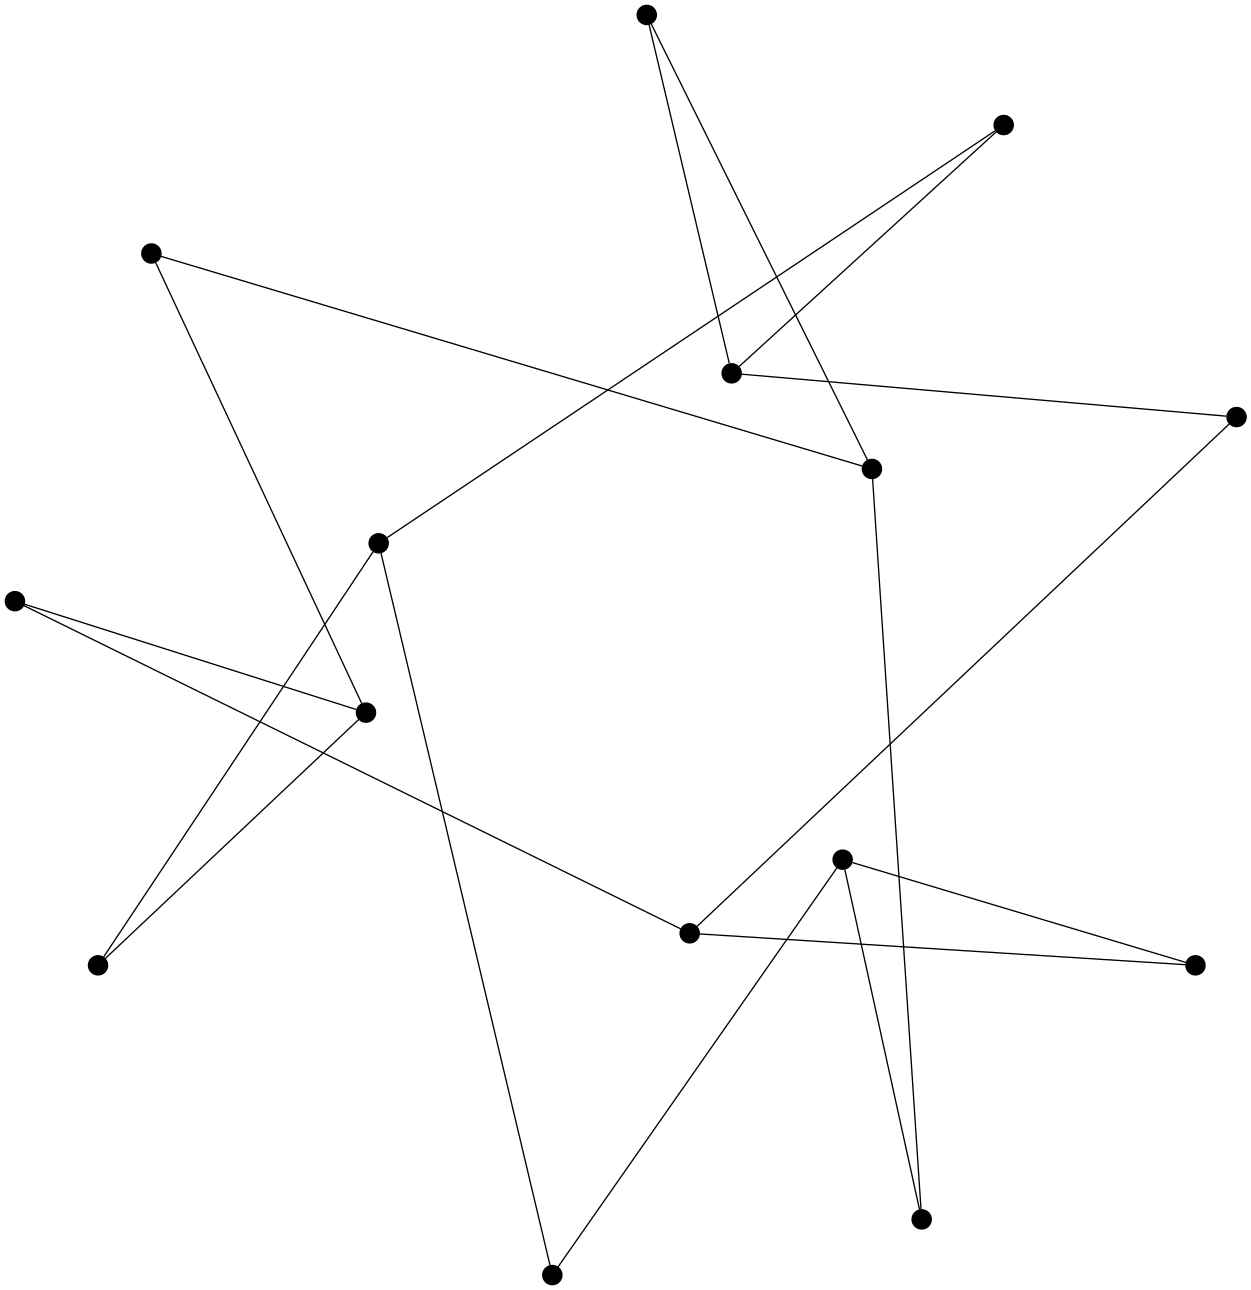
\includegraphics[scale=0.2]{graph_2.png}
    \caption{ (2,3)-регулярный двудольный граф с обхватом 8. }
    \label{be_not_afraid}
\end{figure}

На рисунке \ref{be_not_afraid_2} изображён двудольный граф с обхватом 14, полученный из метаграфа, построенного на основе двудольного графа с обхватом 6 из предыдущего пункта с помощью алгоритма 2, с последующим 7-расширением. Он содержит 42 проверочных и 63 информационных вершины.

\begin{figure}[H]
    \centering
    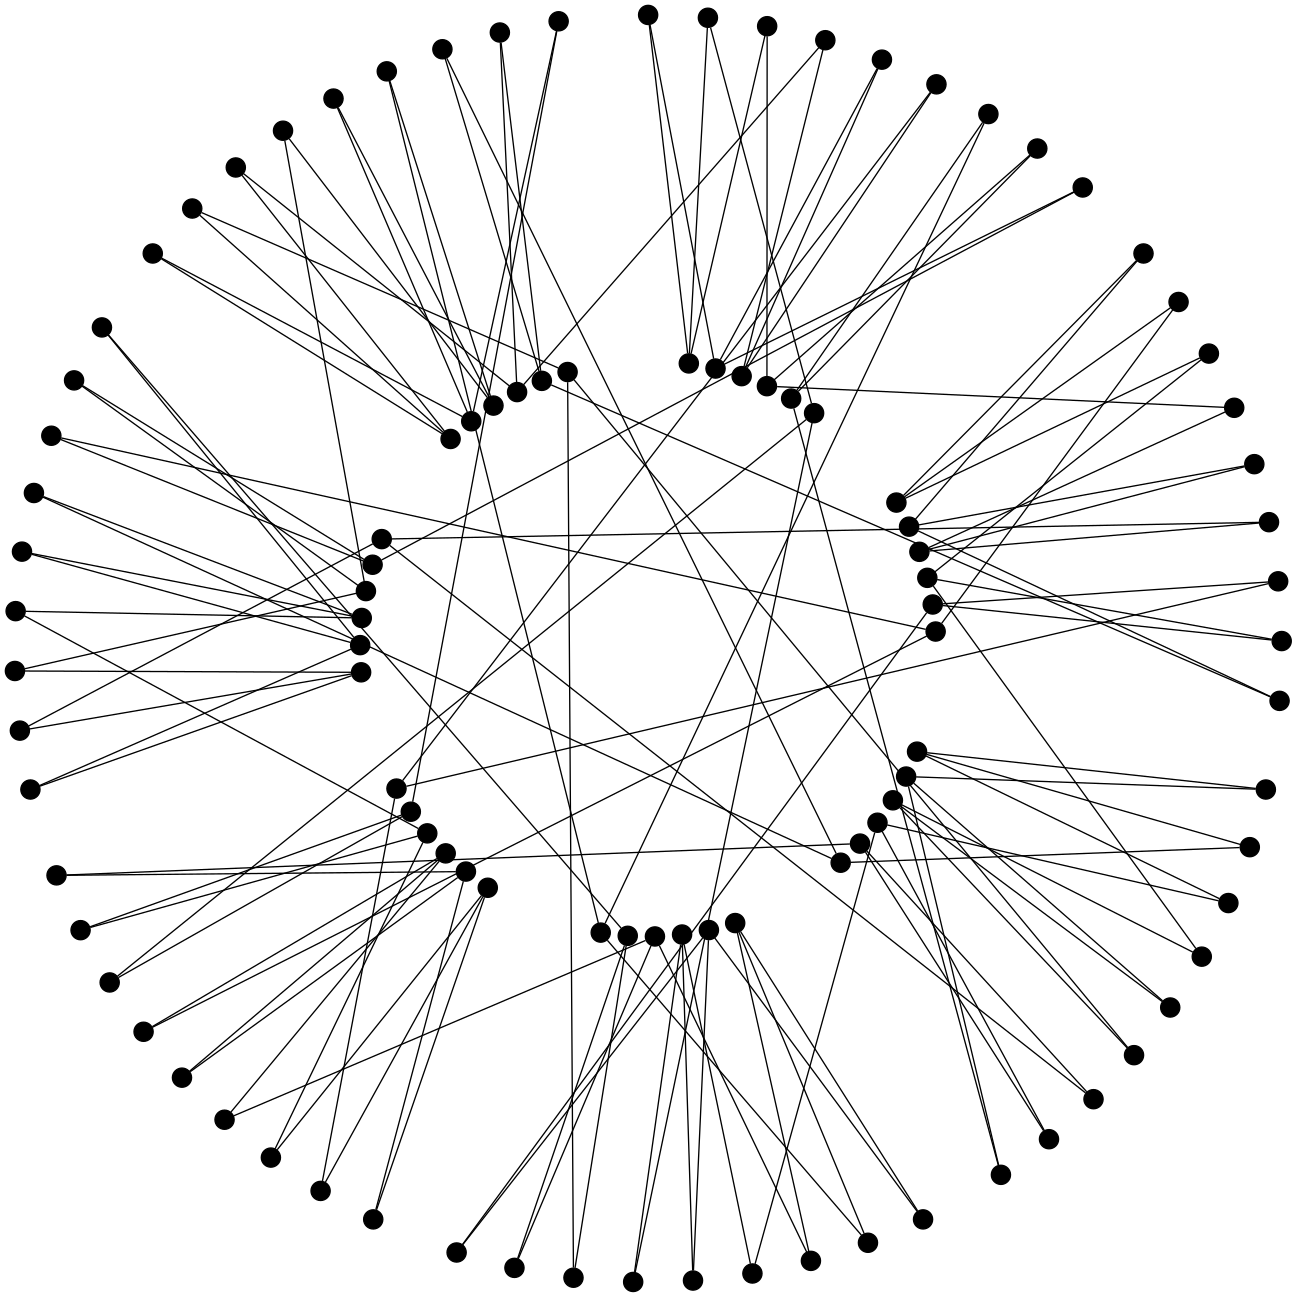
\includegraphics[scale=0.2]{graph_3.png}
    \caption{ (2,3)-регулярный двудольный граф с обхватом 14. }
    \label{be_not_afraid_2}
\end{figure}

\textbf{Замечание.}

Граф с большим обхватом 14 несколькими способами: например построив сначала граф с обхватом 6, а по нему ~-- с обхватом 14, или сначала построить граф с обхватом 12 и по нему с обхватом 14. Доказательство наличия оптимального варианта построения, которое бы породило граф минимального размера, выходит за рамки данной работы, однако мы приведём практическое наблюдение, что лучше минимизировать количество шагов, а при равном количестве шагов, минимизировать размеры более ранних этапов.

\section{Вычислительный эксперимент}

Для оценки характеристик графов, построенных с помощью алгоритма 2. был проведён вычислительный эксперимент.

\textbf{Выбор платформы.}

Для выбора платформы проведения экспериментов были изучены характеристики современных языков программирования. Важным критерием для выбора была производительность, так как задача построения графов большого обхвата вычислительно трудная. Это заставило отказаться от высокоуровневых языков со сложным рантаймом, таких как Python, Java и C\#. Тогда как высокая производительность на этих языках достижима, это требует приложения большого количества усилий, которого можно избежать при использовании языка без рантайма.

Среди современных языков, не содержащих рантаймы были рассмотрены три основных кандидата: C, C++ и Rust. Бенчмарки показывают, что производительность этих языков соизмерима. Язык C был отброшен из-за низкой выразительности, затрудняющей гибкое описание структуры метаграфа. Между C++ и Rust выбор был сделан в пользу последнего из-за более строгой и выразительной системы типов, удобной для описания математических объектов, а так же гарантий безопасности во времени компиляции.

\textbf{Реализация алгоритмов.}

Двудольный граф представлен в виде матрицы логических элементов, строки которой соответствуют проверочным вершинам, а столбцы ~-- информационным. Такое представление не допускает кратных дуг, однако выше было показано, что кратные дуги быстро приводят к уменьшению обхвата метаграфа, так что отказ от них не является проблемой. В листинге \ref{graph_struct} показана реализация графа, а так же методов инициализации пустого графа и добавления дуги в существующий граф.

\begin{lstlisting}[language=Rust, caption={ Структура, описывающая граф и некоторые её методы. }, label=graph_struct]
    #[derive(Clone)]
    pub struct Graph {
        matrix: Matrix<bool>,
    }

    impl Graph {
        pub fn new(control: usize, info: usize) -> Self {
            Self {
                matrix: Matrix::new(info, control),
            }
        }

        pub fn add_edge(&mut self, control: usize, info: usize) {
            self.matrix[(info, control)] = true;
        }
    }
\end{lstlisting}

Для представления отдельной вершины используется тип перечислимый тип, называемый так же Enumeration. Вершина имеет два варианта: Vertex::I ~-- для представления информационных вершин и Vertex::C ~-- для проверочных. В листинге \ref{vertex_enum} показана реализация данного типа.

\begin{lstlisting}[language=Rust, caption={ Перечисление, описывающее вершину графа. }, label=vertex_enum]
    #[derive(PartialEq, Eq, Debug, Hash, Clone, Copy)]
    pub enum Vertex {
        I(usize),
        C(usize),
    }
\end{lstlisting}

Многие приведённые в данной работе алгоритмы основаны на алгоритме поиска в ширину, для реализации которого требуется итерация по вершинам, смежным с данной. Для оптимальной реализации получения последовательности вершин, смежных данной, будем использовать паттерн Итератор. Это позволит избежать дополнительных аллокаций динамической памяти. Структура, описывающая итератор, показана в листинге \ref{iterator_struct}. Она содержит ссылку на граф, для которой необходимо явно указать время жизни, так же называемое lifetime. Это нужно для статического анализа, обеспечивающего защиту от некорректного использования памяти. 

\begin{lstlisting}[language=Rust, caption={ Структура, описывающая итератор по смежным вершинам. }, label=iterator_struct]
    struct AdjacentIter<'a> {
        graph: &'a Graph,
        vertex: Vertex,
        idx: usize,
    }
\end{lstlisting}

Для использования данной структуры в качестве итератора, необходимо реализовать типаж, так же называемый trait, Iterator. Реализация типажа показана в листинге \ref{iterator_impl}. В зависимости от того какой доле принадлежит вершина, ищется следующая дуга, после того, как дуга найдена, возвращается смежная ей вершина из другой доли графа. Если дуга не найдена возвращается значение None перечисления Option, что сигнализирует о завершении работы итератора. 

\begin{lstlisting}[language=Rust, caption={ Реализация типажа Iterator для структуры итератора по смежным вершинам. }, label=iterator_impl]
    impl<'a> Iterator for AdjacentIter<'a> {
        type Item = Vertex;
        fn next(&mut self) -> Option<Self::Item> {
            let res;
            match self.vertex {
                Vertex::I(i) => 'block: {
                    while self.idx < self.graph.control() {
                        if self.graph.has_edge(self.idx, i) {
                            res = Vertex::C(self.idx);
                            break 'block;
                        }

                        self.idx += 1;
                    }

                    return None;
                }
                Vertex::C(c) => 'block: { /* Аналогично */ }
            };
            self.idx += 1;
            Some(res)
        }
    }
\end{lstlisting}

Множество меток в прикладной реализации устроено сложнее, чем неструктурированное множество четвёрок, описанное выше. Вместо этого предлагается использовать структуру типов, описанную в листинге \ref{types}. Одно поколение меток представлено в виде ассоциативного массива, ключами в котором являются вершины, которыми помечены метки, а значениями ~-- пары состоящие из суммы коэффициентов и вершины, на основе которой была сгенерирована метка. Так как в данной реализации не может быть кратных дуг, две вершины однозначно определяют дугу, так что можно избежать хранения дуги. Отдельные поколения меток хранятся в динамическом массиве, индекс в котором соответствует номеру поколения.

\begin{lstlisting}[language=Rust, caption={ Метод генерации одного поколения меток. }, label=types] 
    type LabelGen<const SIZE: usize> = HashMap<
        Vertex,
        Vec<(Eq<SIZE>, Vertex)>
    >;
    type Labels<const SIZE: usize> = Vec<LabelGen<SIZE>>;
\end{lstlisting}

Для генерации множества меток используется метод генерации следующего поколения меток по текущему, описанный в листинге \ref{generate_label_generation}. Он затем вызывается последовательно для всех требуемых поколений, чтобы получить множество всех необходимых меток. 

\begin{lstlisting}[language=Rust, caption={ Метод генерации одного поколения меток. }, label=generate_label_generation]
    fn generate_label_generation(&self, prev_gen: &LabelGen<SIZE>)
        -> LabelGen<SIZE>
    {
        let mut res = HashMap::new();

        for (&vertex, eqs) in prev_gen.iter() {
            for adj in self.graph.adjacent(vertex) {
                let vec = res
                    .entry(adj)
                    .or_insert_with(Vec::new);
                for &(eq, prev_vertex) in eqs.iter() {
                    if prev_vertex == adj {
                        continue;
                    }
                    let new_eq = self.modify_eq(eq, vertex, adj);
                    vec.push((new_eq, vertex));
                }
            }
        }

        res
    }
\end{lstlisting}

Для генерации множества неравенств, поэлементно сравниваются все метки с одинаковым индексом поколения и с одинаковой вершиной, что можно легко сделать при помощи выбранного способа хранения данных. Получившиеся неравенства хранятся в виде массива статической длины SIZE, которая соответствует количеству дуг в графе. В случае, если первое ненулевое слагаемое в левой части не равенства отрицательно, всё неравенство умножается на $-1$, чтобы избежать повторений в множестве не равенств.

Решение системы находится путём подбора значения каждой переменной.

\textbf{Структура эксперимента.} 

Эксперимент состоял из двух основных частей: изучение размеров графов с обхватом 12, полученных расширением полных метаграфов, изучение метаграфов с обхватом больше 12, полученных итеративным методом.

В первой части, к метаграфам с тремя проверочными вершинами и различным количеством информационных применялся алгоритм 2. с различными требуемыми обхватами: 6, 8, 10, 12. Полученная система не равенств решалась с помощью алгоритма 3.

Во второй части, строились графы с обхватом больше 12: 14, 16, 18, 20 с помощью итеративного метода. Они сравнивались с графами с обхватом больше 12, полученными на основе графов с обхватом 6, полученными иными способами.  

\textbf{Результаты эксперимента.}

В Таблице \ref{experiment_label_count_table} представлены количества уникальных не равенств, сгенерированных для различного размера полных метаграфов с различными требуемыми обхватами. Количество информационных вершин метаграфа приведено в заголовке столбца, а требуемый обхват ~-- в первом столбце каждой строки. Отметим, что полное построение системы не равенств для графа с 45 информационными вершинами и обхватом 12  потребовало слишком большого количества памяти, так что вместо этого была только получена оценка размера системы.

\begin{table}[H]
    \centering
    \begin{tabular}{ | c | c | c | c | c | }
        \hline
                   & $|i| = 9$         & $|i| = 15$        & $|i| = 27$      & $|i| = 45$   \\ \hline
        $ l = 6 $  & 108               & 315               & 1'053           & 2'970        \\ \hline
        $ l = 8 $  & 612               & 3'045             & 18'603          & 88'110       \\ \hline
        $ l = 10 $ & 8'766             & 77'385            & 889'434         & 7'181'955    \\ \hline
        $ l = 12 $ & 52'614            & 830'865           & 18'053'334      & $\sim$ 255'000'000 \\ \hline
    \end{tabular}
    \caption{ Размеры систем не равенств для различных метаграфов. }
    \label{experiment_label_count_table}
\end{table}

По этим данным видно, что количество неравенств экспоненциально возрастает с увеличением требуемого обхвата. Что соответствует природе алгоритма поиска в ширину. Количество неравенств так же значительно возрастает вместе с ростом числа информационных вершин. 

\begin{figure}[H]
    \centering
    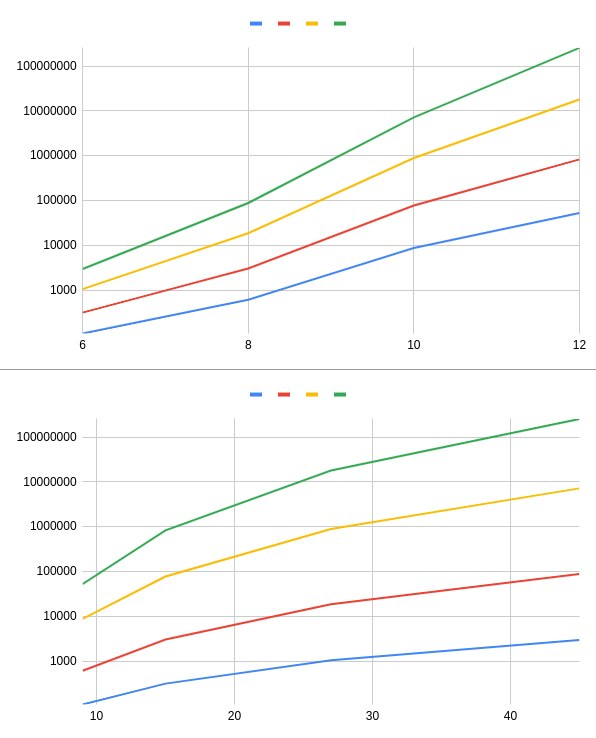
\includegraphics[scale=0.6]{eq_count_plots.jpg}
    \caption{ Графики количества не равенств в зависимости от требуемого обхвата (сверху), количества информационных вершин (снизу). }
    \label{eqs_count_plots}
\end{figure}

На рисунке \ref{eqs_count_plots} изображены графики количества не равенств в зависимости от требуемого обхвата и количества информационных вершин с логарифмической шкалой количества неравенств. На этих графиках видно, что зависимость обхвата действительно экспоненциальна, в то время как зависимость от количества информационных вершин субэкспоненциальна.

В таблице \ref{info_vertex_count_table} показано количество информационных вершин в полученных r-расширениях в зависимости от количества информационных вершин в метаграфе и требуемого обхвата.

\begin{table}[H]
    \centering
    \begin{tabular}{ | c | c | c | c | c | }
        \hline
                   & $|i| = 9$         & $|i| = 15$        & $|i| = 27$      & $|i| = 45$  \\ \hline
        $ l = 6 $  & 126               & 360               & 1134            & 3'195       \\ \hline
        $ l = 8 $  & 549               & 2535              & 14'769          & 68'355      \\ \hline
        $ l = 10 $ & 6'453             & 46'185            & 373'599         & 2'518'875   \\ \hline
        $ l = 12 $ & 21'681            & 226'605           & 3'993'327       &             \\ \hline
    \end{tabular}
    \caption{ Количество информационных вершин в полученных расширениях метаграфов. }
    \label{info_vertex_count_table}
\end{table}

Во второй части эксперимента рассматривались в основном (3,3)-регулярные графы с равным количеством проверочных и информационных вершин. Для построения графов с обхватами 14, 16 и 18 использовалось несколько способов:

1. Построение построение промежуточного графа с обхватом 6, 8 или 10 из полного графа с тремя проверочными и тремя информационными вершинами. Будем обозначать их знаками $G_f^6$, $G_f^8$ и $G_f^10$ соответственно.

2. Построение промежуточного графа с обхватом 6 из метаграфа с одной информационной и одной проверочной вершинами и тремя кратными дугами. Такой метаграф порождает граф с обхватом 6 с семью информационными и семью проверочными дугами. Экспериментально, а именно полным перебором, было показано, что графа с меньшим количеством проверочных вершин и обхватом 6 не существует. Такой метаграф будем обозначать знаком $G_m^6$. Он изображён на рисунке \ref{minimal_girth_6_graph}.

При построении графов с обхватом 14, минимальный результат дал промежуточный граф $G_f^6$, его расширение с обхватом 14 имеет 621 информационную вершину. У расширения метаграфа $G_f^8$ ~-- 693 информационных вершины, у $G_f^{10}$ ~--- 1053, а у $G_m^{6}$ ~-- 917.

\begin{figure}[H]
    \centering
    \begin{picture}(250,200)
        \put(35,165){ \thicklines{ \circle* { 5 } } }
        \bezier{300}(45,165)(45,100)(45,35)
        \bezier{300}(45,165)(60,100)(75,35)
        \bezier{300}(45,165)(90,100)(135,35)
        \put(65,165){ \thicklines{ \circle* { 5 } } }
        \bezier{300}(75,165)(75,100)(75,35)
        \bezier{300}(75,165)(90,100)(105,35)
        \bezier{300}(75,165)(120,100)(165,35)
        \put(95,165){ \thicklines{ \circle* { 5 } } }
        \bezier{300}(105,165)(105,100)(105,35)
        \bezier{300}(105,165)(120,100)(135,35)
        \bezier{300}(105,165)(150,100)(195,35)
        \put(125,165){ \thicklines{ \circle* { 5 } } }
        \bezier{300}(135,165)(135,100)(135,35)
        \bezier{300}(135,165)(150,100)(165,35)
        \bezier{300}(135,165)(180,100)(225,35)
        \put(155,165){ \thicklines{ \circle* { 5 } } }
        \bezier{300}(165,165)(105,100)(45,35)
        \bezier{300}(165,165)(165,100)(165,35)
        \bezier{300}(165,165)(180,100)(195,35)
        \put(185,165){ \thicklines{ \circle* { 5 } } }
        \bezier{300}(195,165)(135,100)(75,35)
        \bezier{300}(195,165)(195,100)(195,35)
        \bezier{300}(195,165)(210,100)(225,35)
        \put(215,165){ \thicklines{ \circle* { 5 } } }
        \bezier{300}(225,165)(135,100)(45,35)
        \bezier{300}(225,165)(165,100)(105,35)
        \bezier{300}(225,165)(225,100)(225,35)
        \put(35,35){ \thicklines{ \circle* { 5 } } }
        \put(65,35){ \thicklines{ \circle* { 5 } } }
        \put(95,35){ \thicklines{ \circle* { 5 } } }
        \put(125,35){ \thicklines{ \circle* { 5 } } }
        \put(155,35){ \thicklines{ \circle* { 5 } } }
        \put(185,35){ \thicklines{ \circle* { 5 } } }
        \put(215,35){ \thicklines{ \circle* { 5 } } }                 
    \end{picture}
    \caption{ Один из минимальных двудольных графов обхватом 6. }
    \label{minimal_girth_6_graph}
\end{figure}
        
При построении расширений с обхватом больше 14 минимальны результат даёт метаграф $G_m^6$ ~-- 1379 информационных вершин для обхвата 16 и 2849 информационных вершин для обхвата 18, однако не существует расширения $G_m^6$ с обхватом 20.

Для обхвата 16 промежуточный метаграф $G_f^6$ порождает расширение с 2178 информационными вершинами, в то время как $G_f^{8}$ ~-- с 1953.

Количество информационных вершин в зависимости от промежуточных метаграфов и требуемого обхвата приведено в таблице \ref{info_vertex_count_table_for_big_girth}. 

\begin{table}[H]
    \centering
    \begin{tabular}{ | c | c | c | c | c | }
        \hline
                   & $G_m^6$      & $G_f^6$     & $G_f^8$     & $G_f^{10}$  \\ \hline
        $ l = 14 $ & 917          & 621         & 693         & 1053        \\ \hline
        $ l = 16 $ & 1379         & 2178        & 1953        & 3483        \\ \hline
        $ l = 18 $ & 2849         & 5409        & 5943        & 7128        \\ \hline
        $ l = 20 $ & Не существует& 12969       & 16527       & 28026       \\ \hline
    \end{tabular}
    \caption{ Количество информационных вершин в полученных расширениях метаграфов. }
    \label{info_vertex_count_table_for_big_girth}
\end{table}

При построении метаграфов с большим количеством информационных вершин тяжело отыскать минимальный граф с обхватом 6, поэтому использовались только расширения полного метаграфа. Расширение промежуточного метаграфа на основе графа с обхватом 6 для требуемого обхвата 14 имеет 68448 информационных вершин, а для требуемого обхвата 16 ~-- 448176 вершин.

Таким образом, вопрос выбора оптимального промежуточного метаграфа для построения графов с большим обхватом нельзя свести к простому правилу. необходим перебор различных вариантов с выбором удачного. Однако эвристикой может служить то, что промежуточные графы меньшего размера обычно порождают меньшие расширения для больших обхватов.

%=======================
\newpage

\addcontentsline{toc}{section}{Заключение}
\section*{Заключение}

В рамках работы были исследована структура циклов в метаграфах, изучены ситуации их соответствия и несоответствия циклам на r-расширениях метаграфов. Был разработан алгоритм поиска кратчайшего цикла на r-расширении метаграфа без построения непосредственного расширения.

На основе алгоритма поиска циклов на метаграфах с фиксированными весами был разработан алгоритм поиска циклов на метаграфах с неизвестными весами, который позволяет понять, возможно ли в принципе получить r-расширение данного метаграфа с   требуемым обхватом и построить систему не равенств, решение которой позволяет получить r-расширение с заданным обхватом. 

Для полученных систем не равенств был разработан алгоритм, определяющий разрешимость и находящий одно из существующих решений. Было показано, что в случае, когда алгоритм поиска циклов в метаграфе с неопределёнными весами не сообщает о принципиальной невозможности построения r-расширения с заданным обхватом, существует решение такой системы не равенств и оно позволяет построить r-расширение с требуемым обхватом. Был найден способ выбора минимального r для найденного решения системы для построения r-расширений с заданным обхватом. 

Так же была изучена структура метаграфов и получены нижние оценки обхватом r-расширений на её основе. На основе этих оценок был сформулирован метод подбора подходящей структуры метаграфа для получения расширения с произвольным заданным обхватом.

Совокупность вышеперечисленных алгоритмов составляет метод построения двудольных графов с заданным обхватом при помощи метаграфов. Данный метод позволяет для любых m и n получить (m,n)-регулярный двудольный граф произвольным заданными обхватом, со сколь угодно большим количеством вершин, однако накладывает ограничение снизу на количество вершин.

Был проведён вычислительный эксперимент для получения практических оценок результатов работы метода. Были оставлены таблицы размеров расширений и размеров множеств неравенств для метаграфов с различным соотношением информационных и проверочных вершин, а так же для различных обхватов. Для обхватов больше 12 применялось несколько итераций метода подбора структуры метаграфа.  

%=======================
\newpage

\addcontentsline{toc}{section}{Литература}
\renewcommand{\refname}{\centering \textbf{Литература}}

\begin{thebibliography}{0}

\bibitem{zemor}
G. Zémor, On Expander Codes, IEEE Trans. on Information theory, IT-47
No 2, (2001) pp. 835–837.
  
\bibitem{johnson}
S.\,J. Johnson,
Introducing Low-Density Parity-Check Codes.
~-- University of Newcastle, Australia, 2006.

\bibitem{gallager}
R.\,G. Gallager,
Low-density parity-check codes
~-- IRE Transactions on Information Theory, 1962.

\bibitem{bruteforce}
Гурский С.\,С., Могилевская Н.\,С.
Задача генерации проверочных матриц ldpc-кодов.
~-- Ростов н/Д : Материалы конференции СИТО, 2021.

\bibitem{protographs}
J. Thorpe,
Low-density parity-check (LDPC) codes constructed from protographs.
~-- JPL, IPN Progress Rep., Aug. 2003, vol. 42–154.

\bibitem{metagraphs}
Арутюнов О.\,В.
Построение (m, n)-регулярных двудольных графов с наибольшим обхватом методом увеличения метаграфов.
~-- Ростов н/Д : Материалы конференции СИТО, 2021.

\bibitem{sidon}
J. Singer,
Perfect difference sets
~-- Brooklyn College, Brooklyn, N. Y, 1966.

\end{thebibliography}

\end{document}